\documentclass[russian,utf8,nocolumnxxxi,nocolumnxxxii]{eskdtext}
\usepackage[T1,T2A]{fontenc}
\usepackage[utf8]{inputenc}
\usepackage{graphicx}
\graphicspath{{pictures/}}
%\usepackage[english,russian]{babel}
\usepackage{amssymb,amsmath}
\usepackage{tikz}
\usepackage{siunitx}
\usepackage[american,cuteinductors,smartlabels]{circuitikz}
\usepackage[backend=biber]{biblatex}
\addbibresource{error_estimation_otchet.bib}
\usepackage[]{hyperref}
\hypersetup{colorlinks=true,}
\usepackage{textcomp}
\newcommand{\No}{\textnumero}
\ESKDdepartment{Федеральное агентство по образованию}
\ESKDcompany{Санкт-Петербургский государственный электротехнический университет "ЛЭТИ"}

\ESKDsignature{Вариант N23}
\ESKDauthor{Рахманов ~М.~А.}
\ESKDchecker{Прокшин~А.~Н.}

\begin{document}
\begin{center}
\hfill \break
\large{МИНОБРНАУКИ РОССИИ}\\
\footnotesize{САНКТ-ПЕТЕРБУРГСКИЙ ГОСУДАРСТВЕННЫЙ}\\ 
\footnotesize{ЭЛЕКТРОТЕХНИЧЕСКИЙ УНИВЕРСИТЕТ}\\
\footnotesize{«ЛЭТИ»ИМ. В.И. УЛЬЯНОВА (ЛЕНИНА)}\\
\hfill \break

 \hfill \break
\normalsize{Кафедра робототехники и автоматизации\\ производственных систем (РАПС)}\\
\hfill\break
\hfill \break
\hfill \break
\hfill \break
\large{Пояснительная записка к Курсовой работе}\\
\largeпо дисциплине "Информатика"\\
\hfill \break
\hfill \break


\hfill \break
\hfill \break
\end{center}
 

\hfill \break
\hfill \break
\begin{center} Санкт-Петербург 2018 \end{center}
\thispagestyle{empty} % выключаем отображение номера для этой страницы
\newpage

{\normalsize{\bf{Содержание}}
\\1. Цель и тема курсовой работы
\\2. Задание на курсовую работу
\\3. Введение
\\4. Исследование функции
\\5. Исследование кубического сплайна
\\6. Задача оптимального распределения неоднородных ресурсов
\\7. Список литературы
\newpage
\normalsize{\bf{Цель курсовой работы:}} уметь применять персональный компьютер и
математические пакеты прикладных программ в инженерной деятельности.
\par
\normalsize{\bf{Тема курсовой работы:}} решение математических задач с использованием
математического пакета "Scilab"или "Reduce-algebra".
\newpage
\begin{center}
 {\large\bf2. Задание на курсовую работу}
\end{center}
\normalsize1. Даны функции $f(x)=\sqrt{3}sin(x)+cos(x),g(x)=cos(2x+\frac{\pi}{3})-1$
\\а)Решить уравнение f(x)=g(x).
\\б)Исследовать функцию h(x)=f(x)-g(x) на промежутке $[0;\frac{5\pi}{6}]$
\\2. Найти коэффициенты кубического сплайна, интерполирующего данные, представленные в векторах:\\
$V_{x}=[0,1.25,2,2.625,4.25]$
$V_{y}=[4,3.925,4.675,4.8,4.956]$\\
Построить на графике функции f(x),полученную после нахождения коэффициентов кубического сплайна. \\
Представить графическое изображение результатов интерполяции исходных данных различными методами с использованием встроенных функций\\ splin(x,y,“natural”), splin(x,y,“clamped”), splin(x,y,“not\_a\_knot”), splin(x,y, “fast”), splin(x,y,“monotone”), interp(xx,x,y,d)\\
3. Решить задачу оптимального распределения неоднородных ресурсов.
Требуется решить следующую задачу оптимального распределения неоднородных ресурсов. Пусть в распоряжении завода железобетонных изделий (ЖБИ) имеется m видов сырья (песок, щебень, цемент) в объемах ${ a_i}$  .Требуется произвести продукцию { n} видов. Дана технологическая норма $c_ij$  требления отдельного i-го вида сырь для изготовления единицы продукции каждого j-го вида. Известна прибыль $\pi_j$  получаема от выпуска единицы продукции j-го вида. Требуется определить, какую продукцию и в каком количестве должен производить завод ЖБИ, чтобы получить максимальную прибыль.
\par
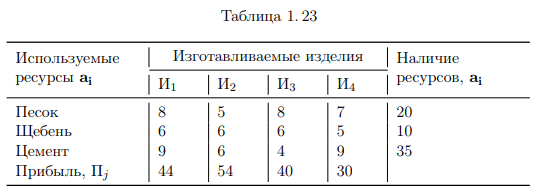
\includegraphics[scale=0.75]{2019-01-09_01-47-19}
\newpage
\begin{center} {\bf3. Введение} \end{center}
\par
\normalsize В современном мире технологие неудержимо летят вперед, с каждым годом электронно вычеслительная техника становиться мощьнее, компактнее и сложнее, а людям приходиться решать все более сложные задачи. С этим людям стали помогать математические пакеты и системы компьютерной алгебры, которые во много раз сокращают время на решение сложнейших задачь, с безчисленым количеством чисел, сейчас такие программы доступны каждому хоть и не все они бесплатные.
\newpage
\begin{center}{\bf4. Исследование функции} \end{center}
\par
\normalsize1. Даны функции:
\\$f(x)=\sqrt{3}sin(x)+cos(x)$\\ 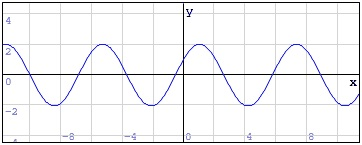
\includegraphics{f(x)}
\\$g(x)=cos(2x+\frac{\pi}{3})-1$\\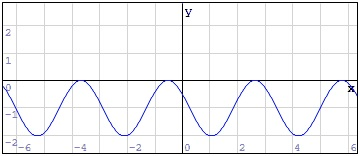
\includegraphics{g(x)}
\\а)Решить уравнение f(x)=g(x).
\\б)Исследовать функцию h(x)=f(x)-g(x) на промежутке $[0;\frac{5\pi}{6}]$\\
{\bfРешение уравнения.}
\\ f(x)=g(x)= f(x)-g(x)=0
\\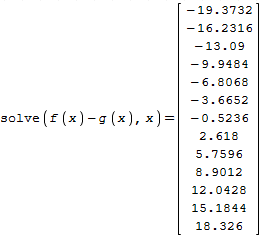
\includegraphics{2019-01-09_02-19-12}
\newpage
{\bf4. Исследование функции}
\par
\normalsize
Корни функции f(x)=g(x) совпадают с корнями иследуемой функции h(x)=f(x)-g(x) и представлены выше.
\\ h(x)=f(x)-g(x)
\\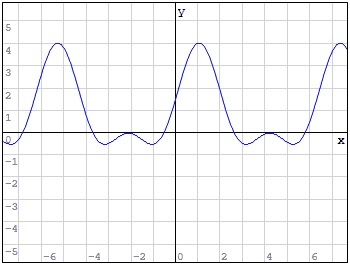
\includegraphics{h(x)=f(x)-g(x)}
\\
\begin{tikzpicture}

\begin{scope}[scale=1]


\draw[thin, ->] (-7,0) -- (7,0) node[right] {$X$};
\draw[thin, ->] (0,-7) -- (0,7) node[left] {$Y$};

\foreach \x\xtext in {-4,-3/x_0,-2,2/x_2,-1/x_1,1,3} 
\draw (\x,0.1) -- (\x,-0.1) node[below] {$\xtext$};
\foreach \y\ytext in {-4,-3,-2,2,-1,1,3,4} 
\draw (0.1,\y) -- (-0.1,\y) node[left] {$\ytext$};


\draw[domain=0:2.3, smooth, blue] plot ({\x},{(3^(1/2))*sin(\x)+cos(\x)});














\end{scope};



\end{tikzpicture}


\newpage
\begin{center}{\bf5. Исследование кубического сплайна.}\end{center}
\par
\normalsize Найти коэффициенты кубического сплайна, интерполирующего данные, представленные в векторах:\\
$V_{x}=[0,1.25,2,2.625,4.25]$
$V_{y}=[4,3.925,4.675,4.8,4.956]$\\
Построить на графике функции f(x),полученную после нахождения коэффициентов кубического сплайна. 
\\Оценить погрешность интерполяции в точке x=3.1. Вычеслить значение функции в точке x=2.1
\\Представить графическое изображение результатов интерполяции исходных данных различными методами с использованием встроенных функций\\ splin(x,y,“natural”), splin(x,y,“clamped”), splin(x,y,“not\_a\_knot”), splin(x,y, “fast”), splin(x,y,“monotone”), interp(xx,x,y,d)\\
\newpage
\begin{center}{\bf Нахождение коэффициентов кубического сплайна.}\\\end{center}
\par
\normalsize
Найдем уравнение сплайна проходящего через пять точкек $(x_{1}, y_{1}),\\
(x_{2}, y_{2}), (x_{3}, y_{3}) и (x_{4}, y_{4})$. Для того чтобы потенциальная энергия изогнутой
металлической линейки(сплайна) принимала минимальное значение,
производная четвертого порядка должна быть равна нулю, значит мы
можем представить сплайн полиномом третьей степени на каждом отрезке
$[x_i, x_{i+1}]$
\\$$F_i(x) = A_{i0} + A_{i1}x + A_{i2}x^2 + A_{i3}x^3, где x \in [x_i, x_{i+1}]$$
\par
\normalsize По такому же принципу состовляем 8 уровнений, по два на каждый участок кривой.
\begin{center}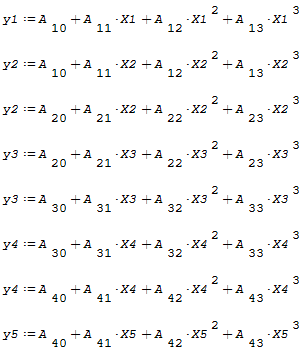
\includegraphics[scale=0.8]{2019-01-09_03-19-11}\end{center}
\par
\newpage
\normalsize
Для того что бы не было излома сплайна, добавляем три уровнения с производными певого порядка, по одному на каждое соединение.
\begin{center}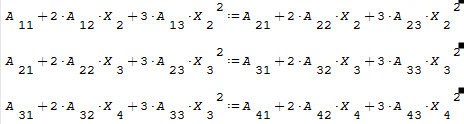
\includegraphics[scale=0.8]{2019-01-09_03-26-45}\end{center}
\par
\normalsize
Для получения одинакового изгиба с каждой стороны стыков, добавляем три уровнения с производными второго порядка.
\begin{center}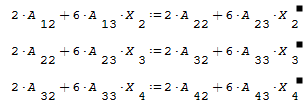
\includegraphics[scale=0.8]{2019-01-09_03-31-08}\end{center}
\par
\normalsize
Добавим уровнения отвечающие за положение концов сплайна, в нашем случае они оставлены свободно.
\begin{center}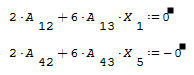
\includegraphics[scale=0.8]{2019-01-09_03-34-49}\end{center}
\newpage
\par
\normalsize
Таким образов были найдены 16 уровнений из которых можно составить матрицу размерностью 16х16. С ее помощью, решая матричное уровнение, находим коофиценты кубического сплайна.
\begin{center}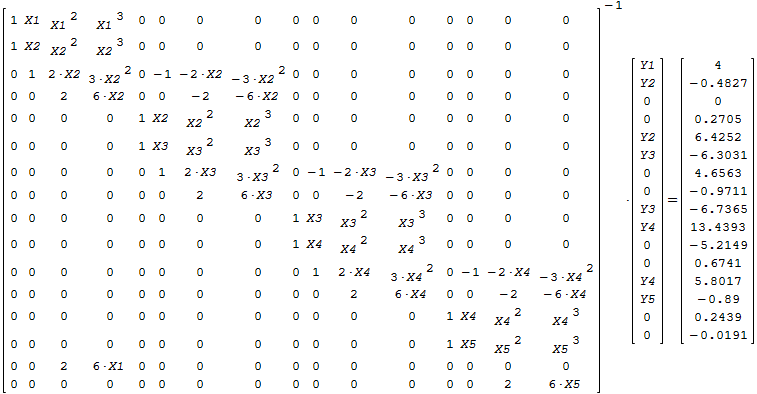
\includegraphics[scale=0.6]{2019-01-09_03-36-31}\end{center}
\par
\normalsize
Получаем окончательное уровнение сплайна.
\begin{center}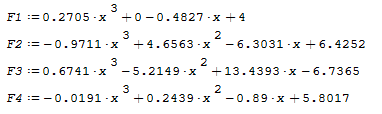
\includegraphics[scale=0.75]{2019-01-09_03-42-54}\end{center}
\newpage
\begin{center}{\bf построение кубического сплайна.}\\\end{center}
\begin{tikzpicture}

\begin{scope}[scale=2]


\draw[thin, ->] (0,0) -- (7,0) node[right] {$X$};
\draw[thin, ->] (0,0) -- (0,7) node[left] {$Y$};

\foreach \x\xtext in {,2,1,3} 
\draw (\x,0.1) -- (\x,-0.1) node[below] {$\xtext$};
\foreach \y\ytext in {2,1,3,4} 
\draw (0.1,\y) -- (-0.1,\y) node[left] {$\ytext$};


\draw[domain=0:1.25, smooth, blue] plot ({\x},{(0.2705*(\x)*(\x)*(\x))+0-(0.4827*(\x))+4});
\draw[domain=1.25:2, smooth, red] plot ({\x},{(-0.9711*(\x)*(\x)*(\x))+(4.6563*(\x)*(\x))-(6.3031*(\x))+6.4252});
\draw[domain=2:2.625, smooth,green] plot ({\x},{(0.6741*(\x)*(\x)*(\x))-(5.2149*(\x)*(\x))+(13.4393*(\x))-6.7365});
\draw[domain=2.625:4.25, smooth, violet] plot ({\x},{(-0.0191*(\x)*(\x)*(\x))+(0.2439*(\x)*(\x))-(0.89*(\x))+5.8017});

\end{scope};



\end{tikzpicture}







\end{document}